\documentclass[tikz,border=4pt]{standalone}
\usepackage{ctex}\usepackage{amsmath}
\begin{document}
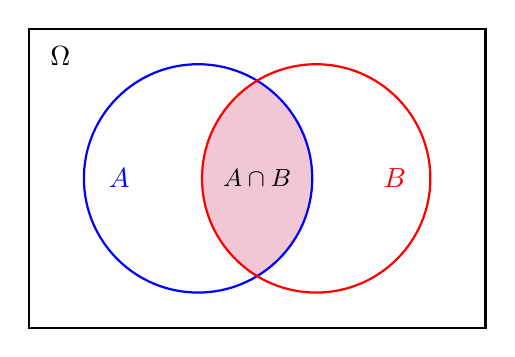
\begin{tikzpicture}
\draw[thick] (-2.9,-1.9) rectangle (2.9,1.9); \node at (-2.5,1.55){$\Omega$};
\begin{scope}\clip (-0.75,0) circle(1.45);\fill[purple!22] (0.75,0) circle(1.45);\end{scope}
\draw[blue,thick] (-0.75,0) circle(1.45); \node[blue] at (-1.75,0){$A$};
\draw[red,thick] (0.75,0) circle(1.45); \node[red] at (1.75,0){$B$};
\node at (0,0){\small $A\cap B$};
\end{tikzpicture}
\end{document}
